\section{Experiments}
\label{sec:joint-experiments}
In the time given, our model did not produce competitive results. Thus, instead of an evaluation in
the fashion of \cref{sec:gmm-experiments}, we discuss the weaknesses of the results on the basis of
visual inspection and illustrative results on data set C~(\cref{subsubsec:gmm-data-c}) in
\cref{subsec:joint-experiment-c} followed by a discussion of the reasons for a continuation of the
work on the model in \cref{subsec:joint-continuation}. The results have been produced with the
parameter settings in \cref{tab:joint-experiments-par}, but the model stably reproduces the same
behavior over a wide parameter range. Due to the lack of a gold standard, which is necessary for an
automated evaluation, the set of parameters have been estimated by visual inspection of the results.
\begin{table}
    \centering
    \renewcommand*{\arraystretch}{1.2}
    \begin{tabular}{l|ccccccc}
        \toprule
        Parameter &  
        $c_{\text{opp}}$ &
        $w_{\text{det}}$ & 
        $w_{\text{count}}$ & 
        $w_{\text{dis}}$ & 
        $w_{\text{div}}$ & 
        $w_{\text{move}}$ & 
        $w_{\text{app}}$ \\ \hline
        Value &  $60000$ & $10$ & $10$ & $1000$ & $10$  & $10$ & $1000$ \\
        \bottomrule
    \end{tabular}
    \renewcommand*{\arraystretch}{1.0}
    \caption[Parameter settings for joint segmentation and tracking]{Parameter settings for joint segmentation and tracking. The high value for the
        opportunity cost $c_{\text{opp}}$ should result in each conflict set containing one active
        region. However, as illustrated by \cref{tab:joint-tracking-result}, regions are falsely
        deactivated. This might hint at an implementation bug.}
    \label{tab:joint-experiments-par}
\end{table}

\subsection{Evaluation of Data Set C}
\label{subsec:joint-experiment-c}
The joint segmentation and tracking method consists of two critical building blocks: The
segmentation and the tracking. In the following, we first inspect the oversegmentation in
\cref{subsubsec:joint-experiment-oversegmentation} before we evaluate the tracking result on this
oversegmentation to determine the shortcomings of our method.

\subsubsection{Oversegmentation}
\label{subsubsec:joint-experiment-oversegmentation}
A good initial oversegmentation result is vital to the overall tracking result. In particular, cells
are potentially oversegmented, but -- by no means -- undersegmented. As illustrated by
\cref{fig:joint-experiment-overseg-a,fig:joint-experiment-overseg-b}, the initial oversegmentation
fulfills this requirement in most cases and fails only a few times, as indicated by orange and pink
ellipses in the overlay images for pixel classification and oversegmentation errors examples
respectively.
\begin{figure}
    \begin{subfigure}[t]{0.48\textwidth}
        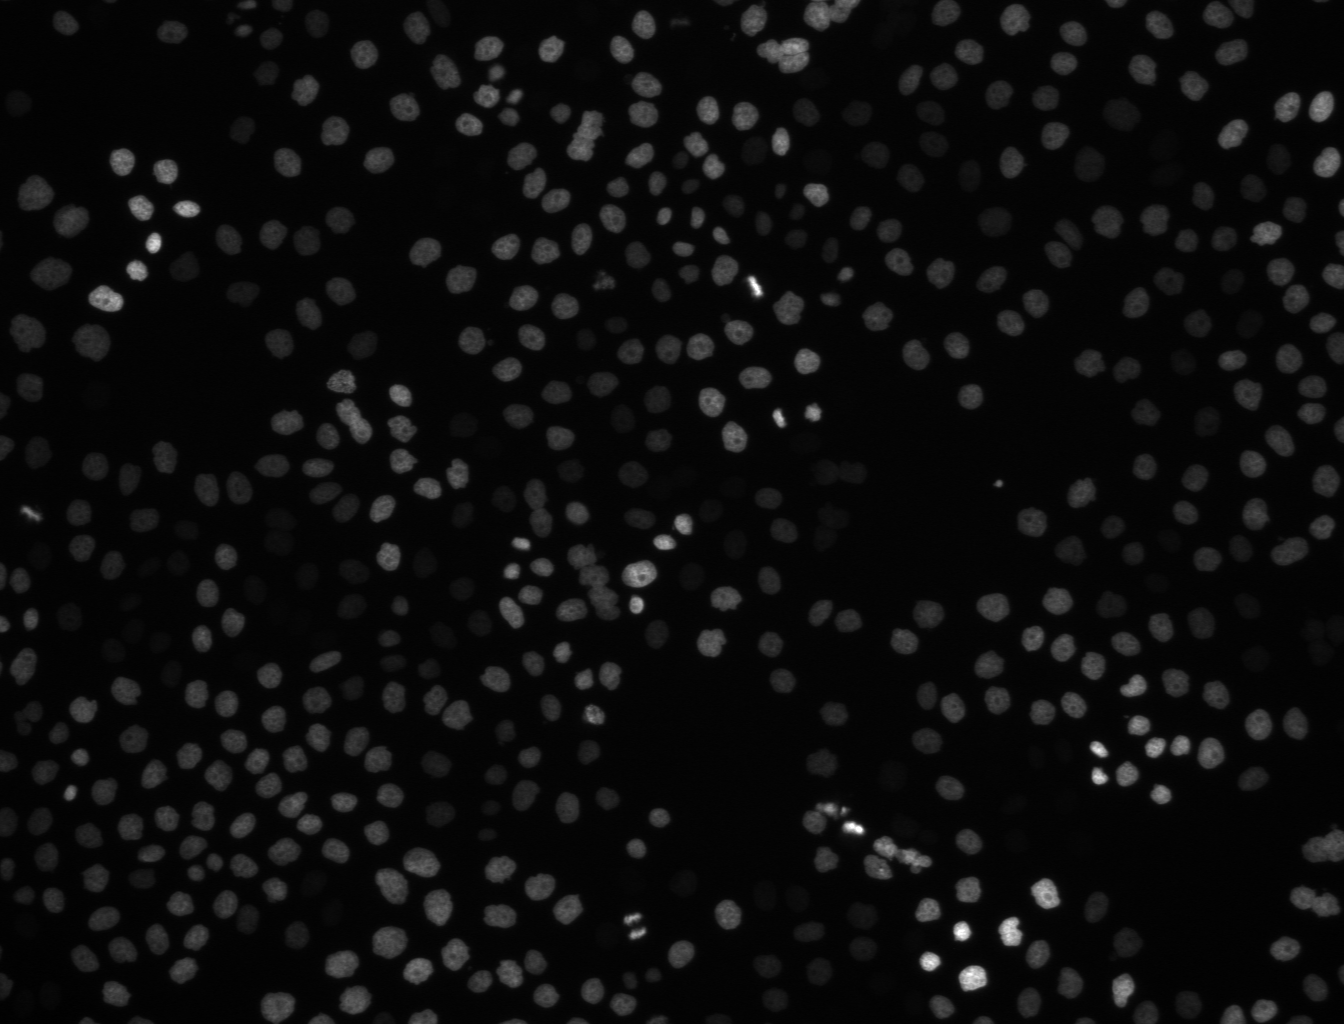
\includegraphics[width=\textwidth]{images/joint/overseg/75/raw.png}
        \caption{Raw data.}
    \end{subfigure}
    \hfill
    \begin{subfigure}[t]{0.48\textwidth}
        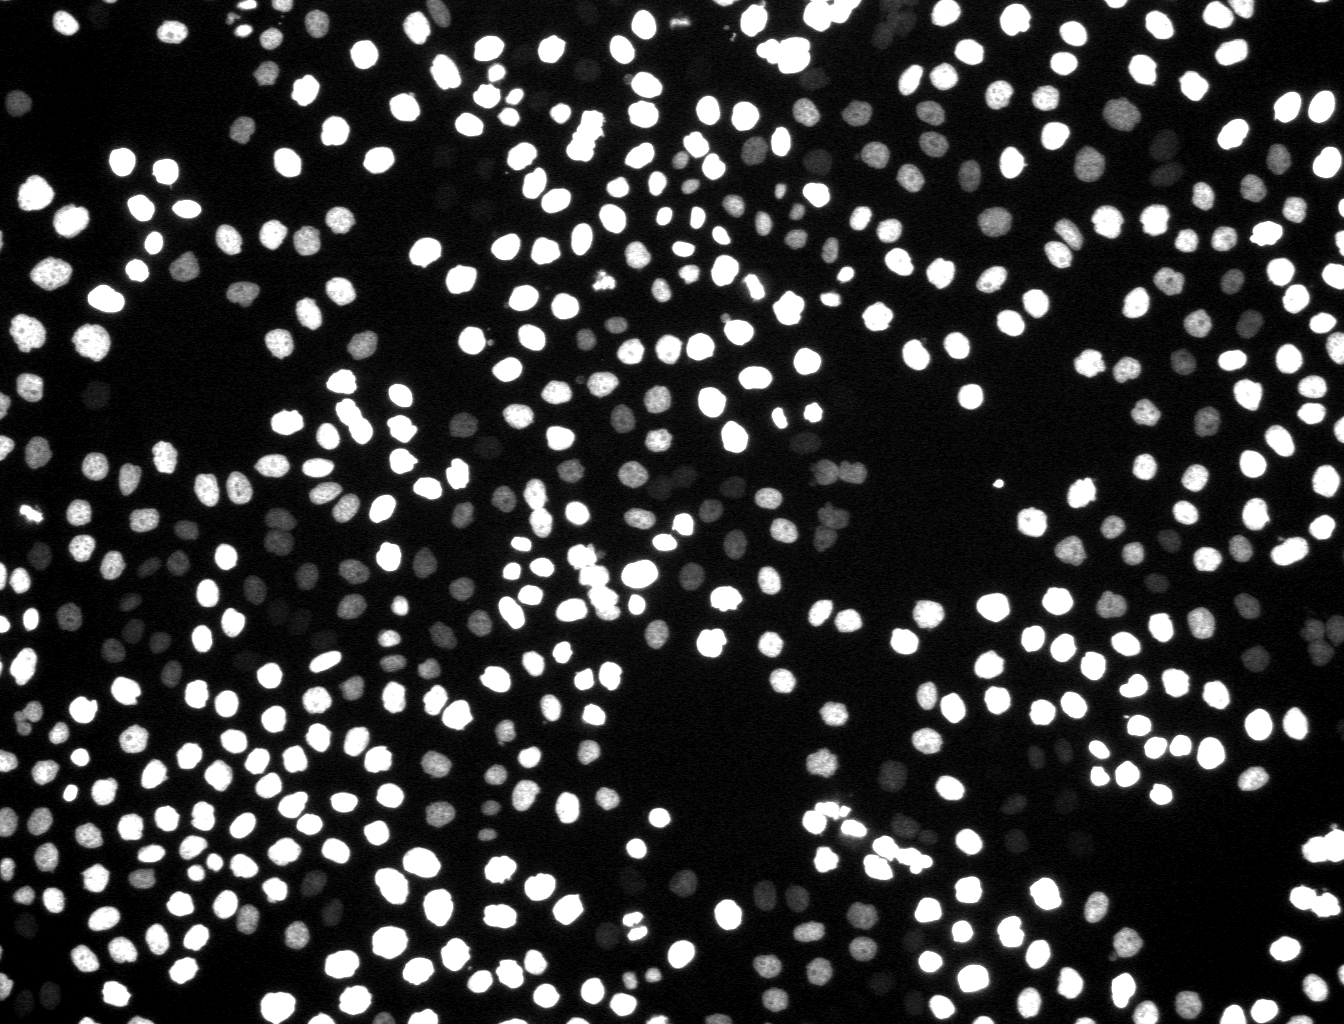
\includegraphics[width=\textwidth]{images/joint/overseg/75/raw_high_contrast.png}
        \caption{Raw data - enhanced contrast.}
    \end{subfigure}
    \\
    \begin{subfigure}[t]{0.48\textwidth}
        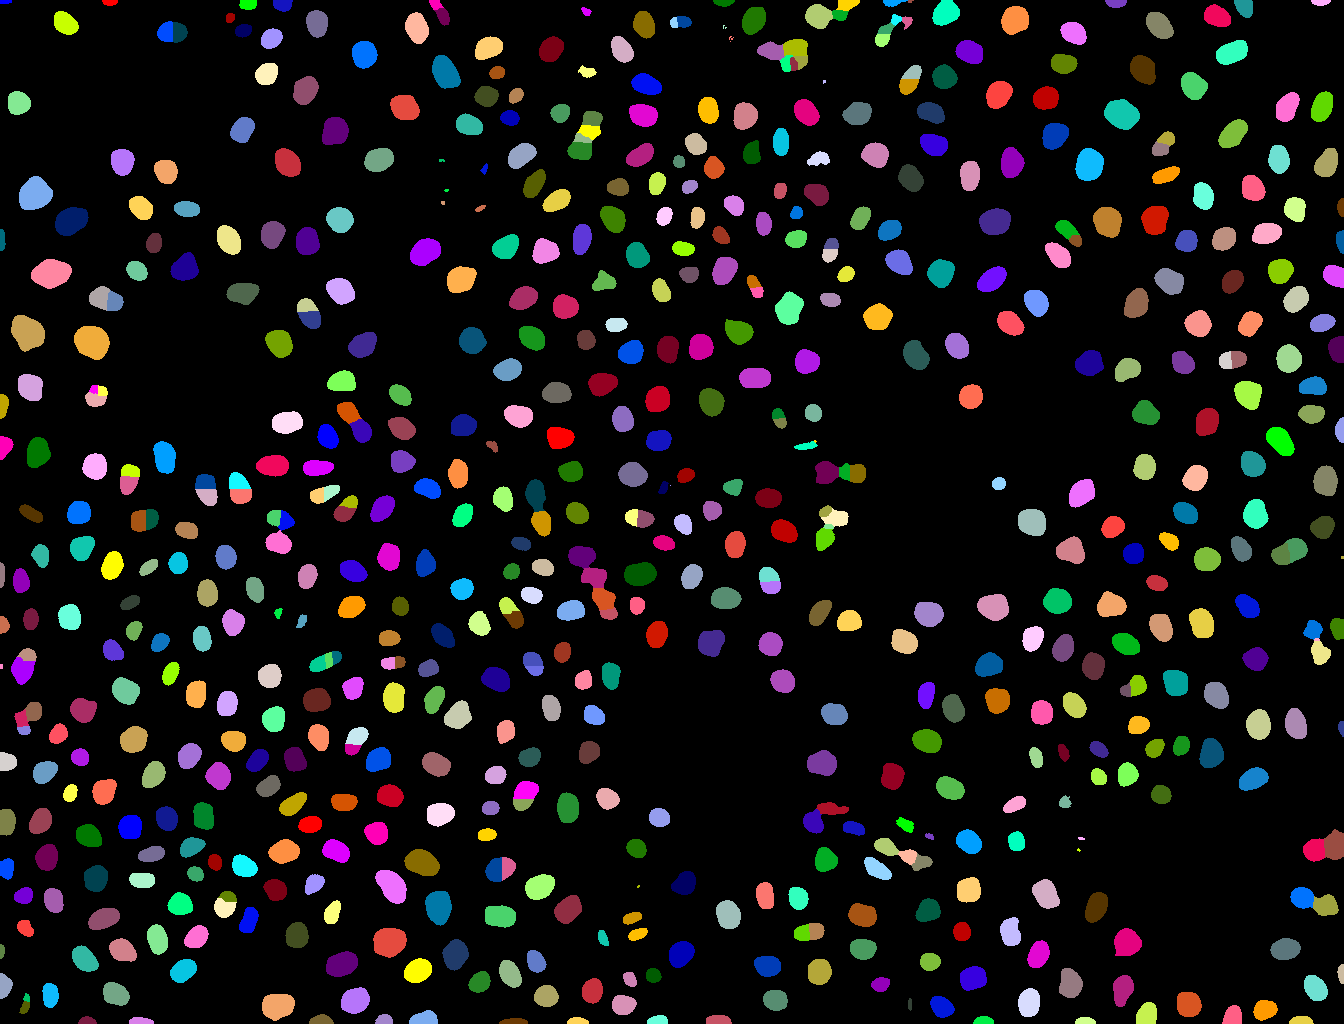
\includegraphics[width=\textwidth]{images/joint/overseg/75/colored.png}
        \caption{Initial oversegmentation.}
    \end{subfigure}
    \hfill
    \begin{subfigure}[t]{0.48\textwidth}
        \begin{tikzpicture}
            \node[anchor=south west,inner sep=0] (image) at (0,0)
            {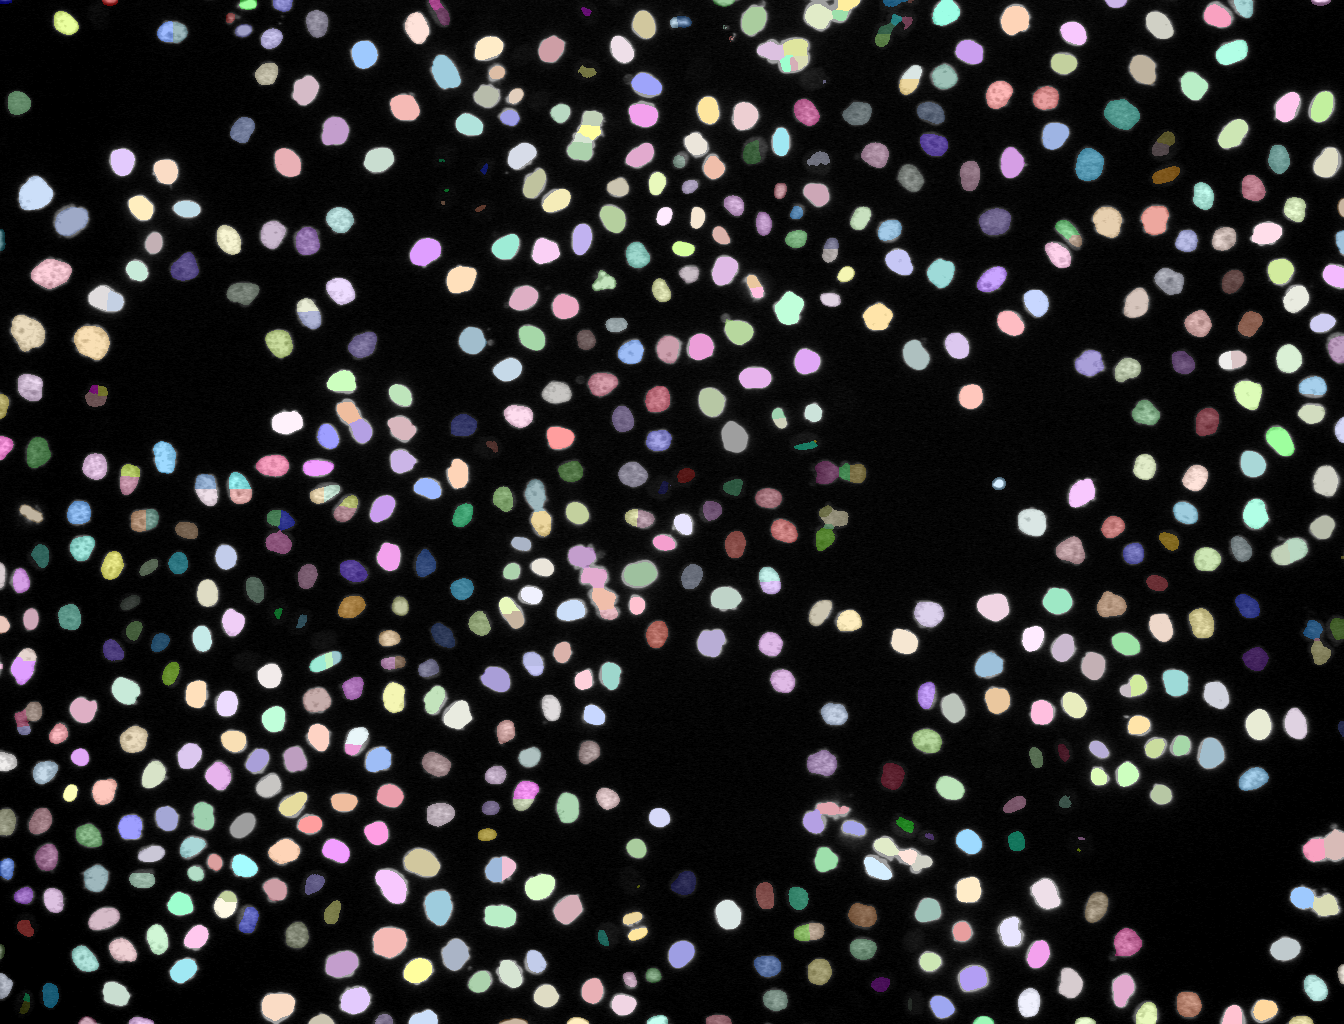
\includegraphics[width=\textwidth]{images/joint/overseg/75/overlay.png}};
            \begin{scope}[x={(image.south east)},y={(image.north west)}]
                \coordinate (c1) at (0.65,0.18);
                \coordinate (c2) at (0.69,0.16);
                \node[thick,draw,ellipse,fill opacity=0,color=magenta, fit=(c1) (c2), scale=0.4,
                xshift=1mm,yshift=-1mm] {};
                \coordinate (c3) at (0.8,0.17);
                \coordinate (c4) at (0.81,0.18);
                \node[thick,draw,ellipse,fill opacity=0,color=orange, fit=(c3) (c4), scale=0.5] {};
                \coordinate (c5) at (0.33,0.81);
                \coordinate (c6) at (0.36,0.83);
                \node[thick,draw,ellipse,fill opacity=0,color=orange, fit=(c5) (c6), scale=0.6] {};
            \end{scope}
        \end{tikzpicture}
        \caption{Overlay of the initial oversegmentation over raw data with enhanced contrast.}
    \end{subfigure}
    \caption[Initial oversegmentation for frame $75$ of data set C]{Initial oversegmentation for
        frame $75$ of data set C: For better distinguishability of the segments, a random color map
        has been applied to the segments in the bottom row.}
    \label{fig:joint-experiment-overseg-a}
\end{figure}

\begin{figure}
    \begin{subfigure}[t]{0.48\textwidth}
        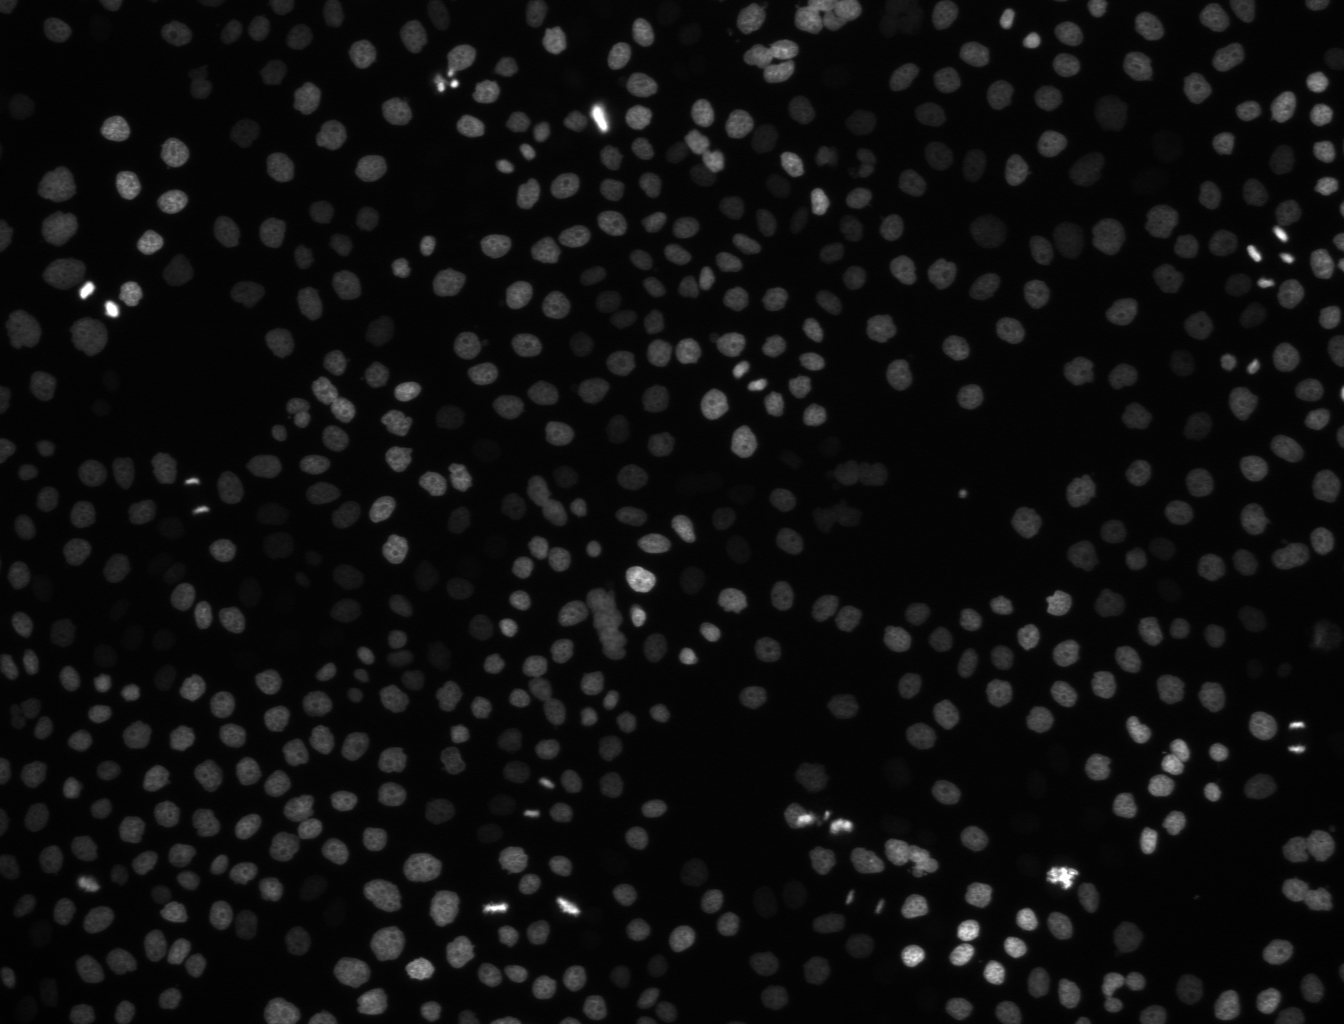
\includegraphics[width=\textwidth]{images/joint/overseg/85/raw.png}
        \caption{Raw data.}
    \end{subfigure}
    \hfill
    \begin{subfigure}[t]{0.48\textwidth}
        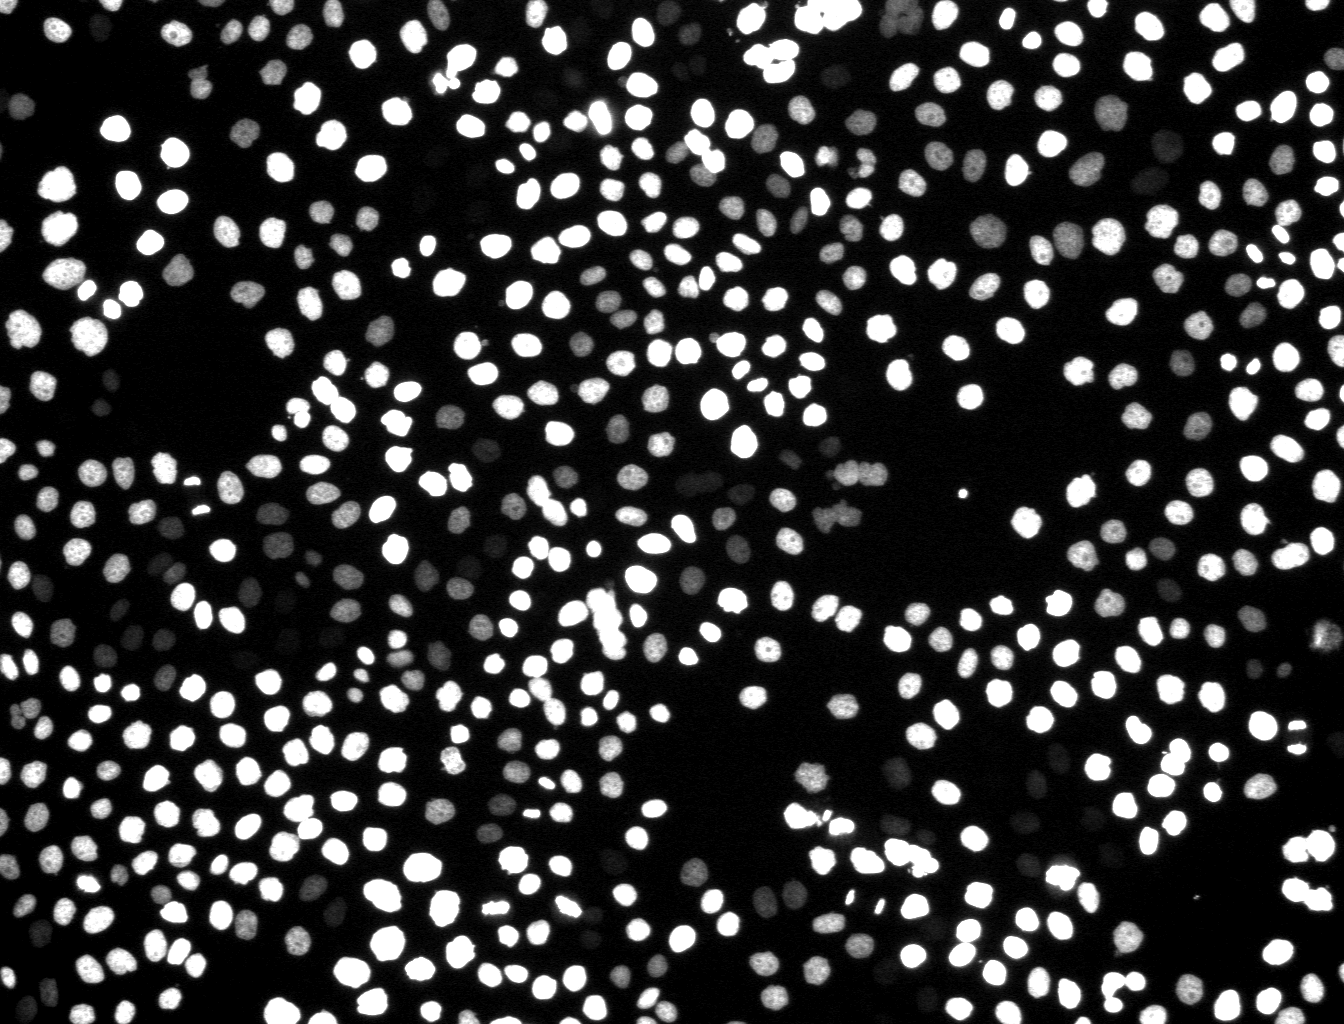
\includegraphics[width=\textwidth]{images/joint/overseg/85/raw_high_contrast.png}
        \caption{Raw data - enhanced contrast.}
    \end{subfigure}
    \\
    \begin{subfigure}[t]{0.48\textwidth}
        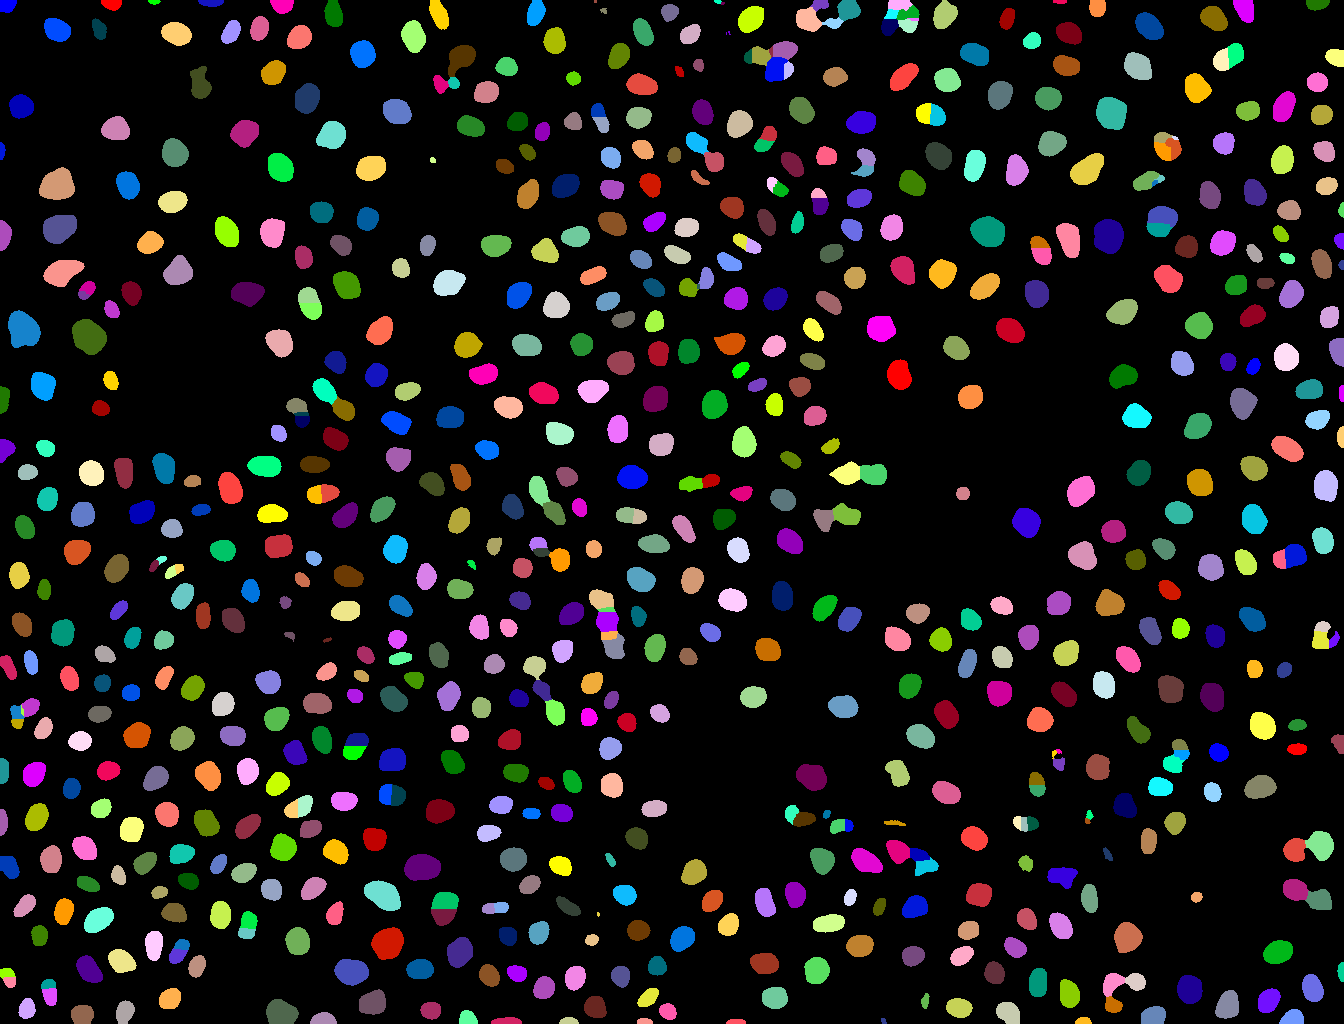
\includegraphics[width=\textwidth]{images/joint/overseg/85/colored.png}
        \caption{Initial oversegmentation.}
    \end{subfigure}
    \hfill
    \begin{subfigure}[t]{0.48\textwidth}
        \begin{tikzpicture}
            \node[anchor=south west,inner sep=0] (image) at(0,0)
            {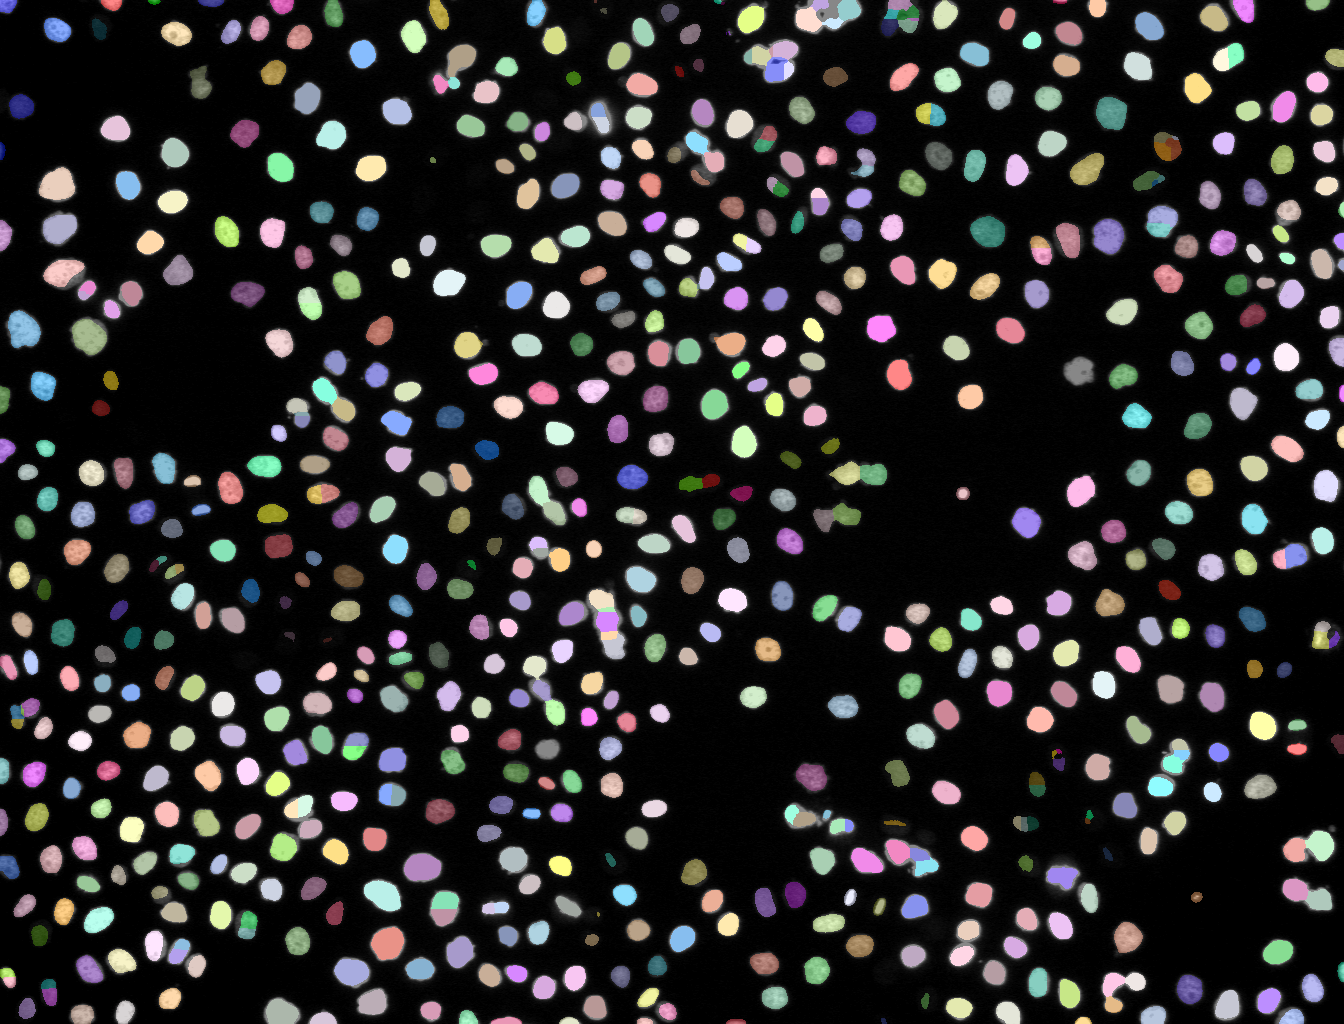
\includegraphics[width=\textwidth]{images/joint/overseg/85/overlay.png}};
            \begin{scope}[x={(image.south east)},y={(image.north west)}]
                % \draw[help lines,xstep=.1,ystep=.1] (0,0) grid (1,1);
                % \foreach \x in {0,2,...,8} { \node [anchor=north] at (\x/10,0) {0.\x}; }
                % \foreach \y in {0,2,...,8} { \node [anchor=east] at (0,\y/10) {0.\y}; }
                \coordinate (c1) at (0.87,0.25);
                \coordinate (c2) at (0.88,0.28);
                \node[thick,draw,ellipse,fill opacity=0,color=magenta, fit=(c1) (c2),scale=0.5,yshift=0mm] {};
                \coordinate (c3) at (0.445,0.105);
                \coordinate (c4) at (0.45,0.107);
                \node[thick,draw,ellipse,fill opacity=0,color=orange, fit=(c3) (c4),scale=0.35] {};
                \coordinate (c5) at (0.32,0.845);
                \coordinate (c6) at (0.325,0.855);
                \node[thick,draw,ellipse,fill opacity=0,color=orange, fit=(c5) (c6),scale=0.35,yshift=-1mm] {};
            \end{scope}
        \end{tikzpicture}
        \caption{Overlay of the initial oversegmentation over raw data with enhanced contrast.}
    \end{subfigure}
    \caption[Initial oversegmentation for frame $85$ of data set C]{Initial oversegmentation for
        frame $85$ of data set C: For better distinguishability of the segments, a random color map
        has been applied to the segments in the bottom row.}
    \label{fig:joint-experiment-overseg-b}
\end{figure}
Furthermore, while the merging algorithm not being sophisticated, the segments still are merged into
reasonable regions in the region merging~(\cf \cref{tab:joint-region-merging-examples}). Overall, the oversegmentation result forms
a legitimate basis for the subsequent tracking.
\begin{table}
    \centering
    \begin{tabular}{cccc}
        \toprule
        \multicolumn{1}{c}{Raw} & \multicolumn{1}{c}{Segments} & \multicolumn{1}{c}{Regions} & \multicolumn{1}{c}{Connected Component} \\ \midrule
        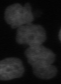
\includegraphics[width=0.15\textwidth]{images/joint/overseg/75/01/raw.png}
        & 
\includegraphics[width=0.15\textwidth]{images/joint/overseg/75/01/colored00.png}
        & 
\includegraphics[width=0.15\textwidth]{images/joint/overseg/75/01/colored01_all.png}
        & 
\includegraphics[width=0.15\textwidth]{images/joint/overseg/75/01/colored02.png} \\
        
\includegraphics[width=0.15\textwidth]{images/joint/overseg/75/02/raw.png}
        & 
\includegraphics[width=0.15\textwidth]{images/joint/overseg/75/02/colored00.png}
        & 
\includegraphics[width=0.15\textwidth]{images/joint/overseg/75/02/colored01_all.png}
        & 
\includegraphics[width=0.15\textwidth]{images/joint/overseg/75/02/colored02.png} \\
        % 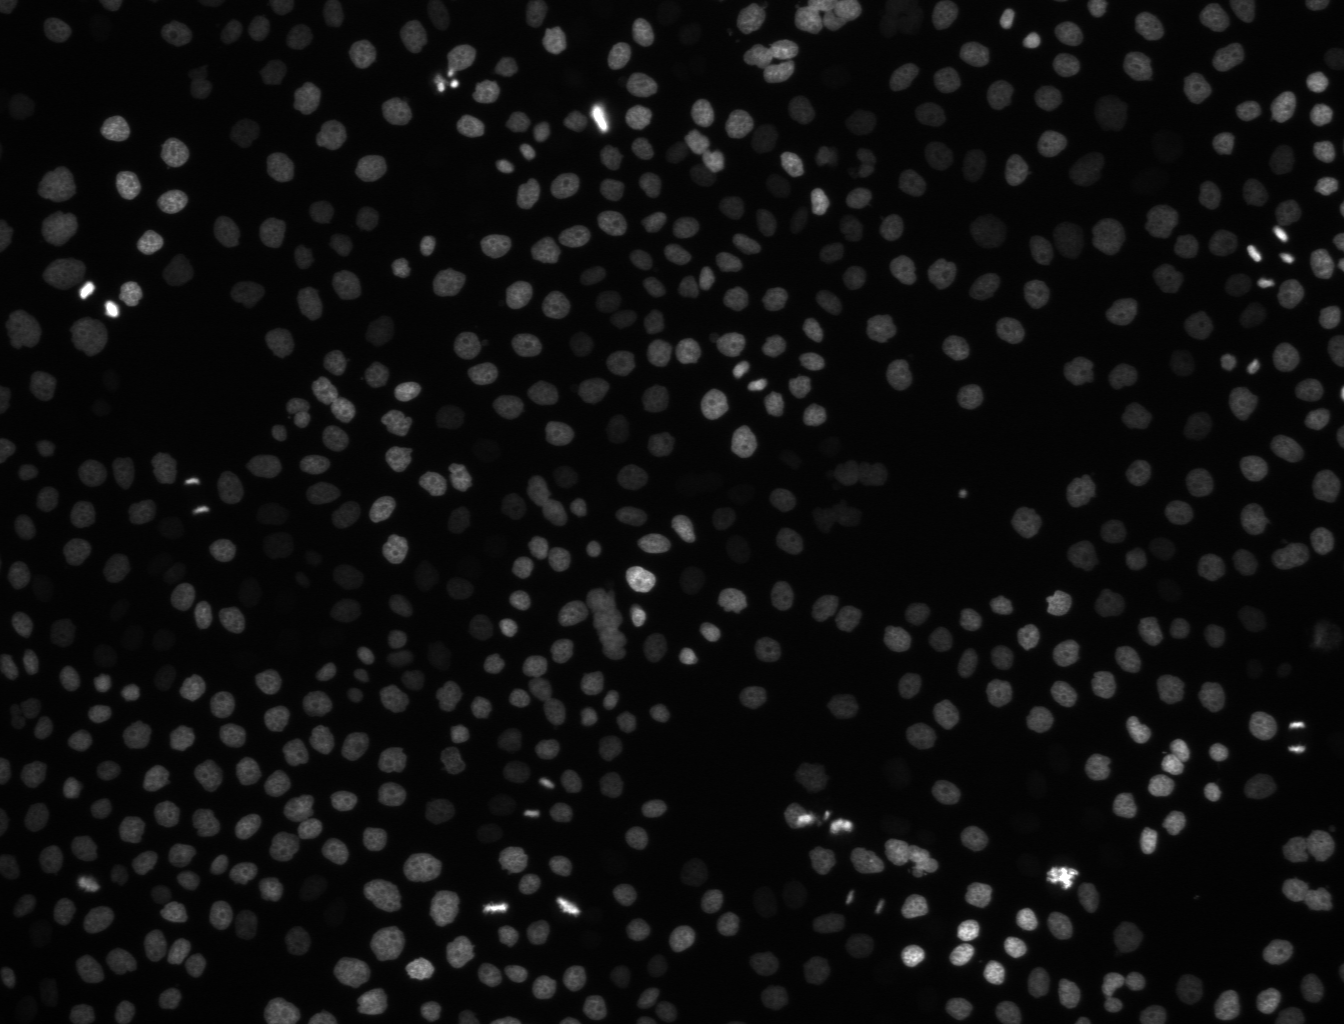
\includegraphics[width=0.15\textwidth]{images/joint/overseg/85/01/raw.png}
        % & 
\includegraphics[width=0.15\textwidth]{images/joint/overseg/85/03/colored00.png}
        % & 
\includegraphics[width=0.15\textwidth]{images/joint/overseg/85/03/colored01_all.png}
        % & 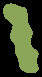
\includegraphics[width=0.15\textwidth]{images/joint/overseg/85/01/colored02.png} \\
        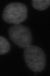
\includegraphics[width=0.15\textwidth]{images/joint/overseg/85/02/raw.png}
        & 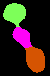
\includegraphics[width=0.15\textwidth]{images/joint/overseg/85/02/colored00.png}
        & % 
\includegraphics[width=0.15\textwidth]{images/joint/overseg/85/02/colored01_all.png}
        & 
\includegraphics[width=0.15\textwidth]{images/joint/overseg/85/02/colored01.png} \\
        \bottomrule
    \end{tabular}
    \caption[Region merging examples]{Region merging examples: The region merging reliably merges in
        a manner that forms new regions that are likely to be cells.  Here, a random color map is
        applied for better distinguishability of regions. If, like in the lowermost row
        where no intermediate regions exist,
        any merging would produce poor cell regions, no action is taken. The connected component is
        the union of all segments and is always a valid segmentation hypothesis by construction.}
    \label{tab:joint-region-merging-examples}
\end{table}



\subsubsection{Tracking Results}
\label{subsubsec:joint-experiment-tracking}
Three subsequent frames of the tracking result, based on the oversegmentation above, are shown in
\cref{fig:joint-tracking-result}. In general, the tracking result looks promising. When it comes to
challenging and more interesting connected components, however, the joint segmentation and tracking
fails. An example for this is indicated by a red ellipse in \cref{fig:joint-tracking-result} and
examined more closely in \cref{tab:joint-tracking-result}.
\begin{figure}
    \begin{subfigure}[t]{0.3\textwidth}
        \begin{tikzpicture}
            \node[anchor=south west,inner sep=0] (image) at(0,0)
            {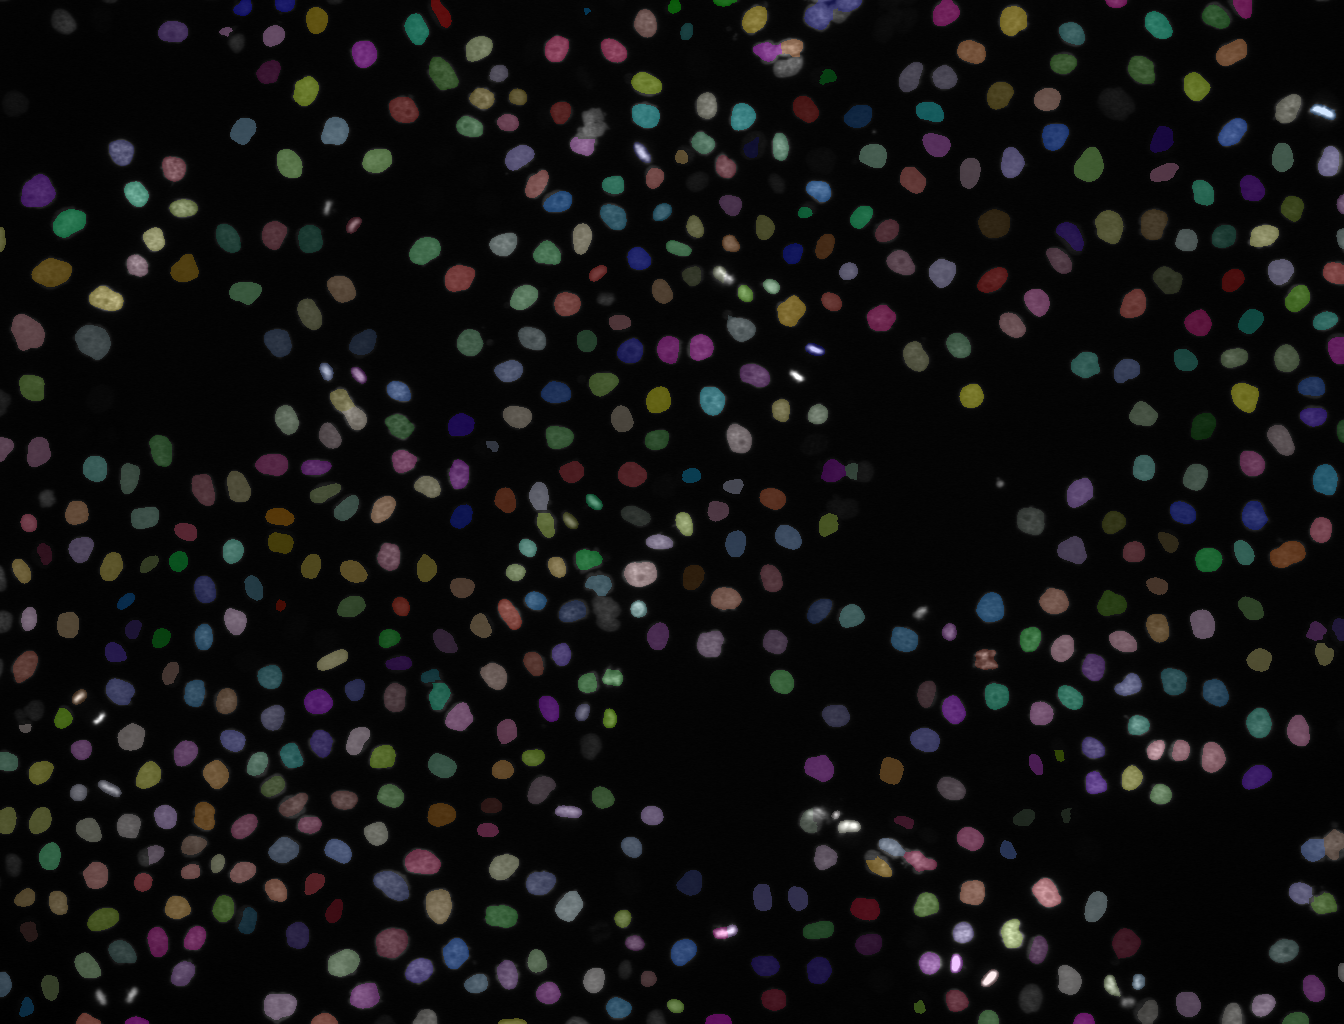
\includegraphics[width=1.0\textwidth]{images/joint/tracking/77_seg_overlay.png}};
            \begin{scope}[x={(image.south east)},y={(image.north west)}]
                \coordinate (c1) at (0.45,0.39);
                \coordinate (c2) at (0.45,0.44);
                \node[thick,draw,ellipse,fill opacity=0,color=red, fit=(c1)
                (c2),scale=0.4,yshift=-0.5mm, opacity=0.7] {};
            \end{scope}
        \end{tikzpicture}
        \caption{$t=77$}
    \end{subfigure}
    \hfill
    \begin{subfigure}[t]{0.3\textwidth}
        \begin{tikzpicture}
            \node[anchor=south west,inner sep=0] (image) at(0,0)
            {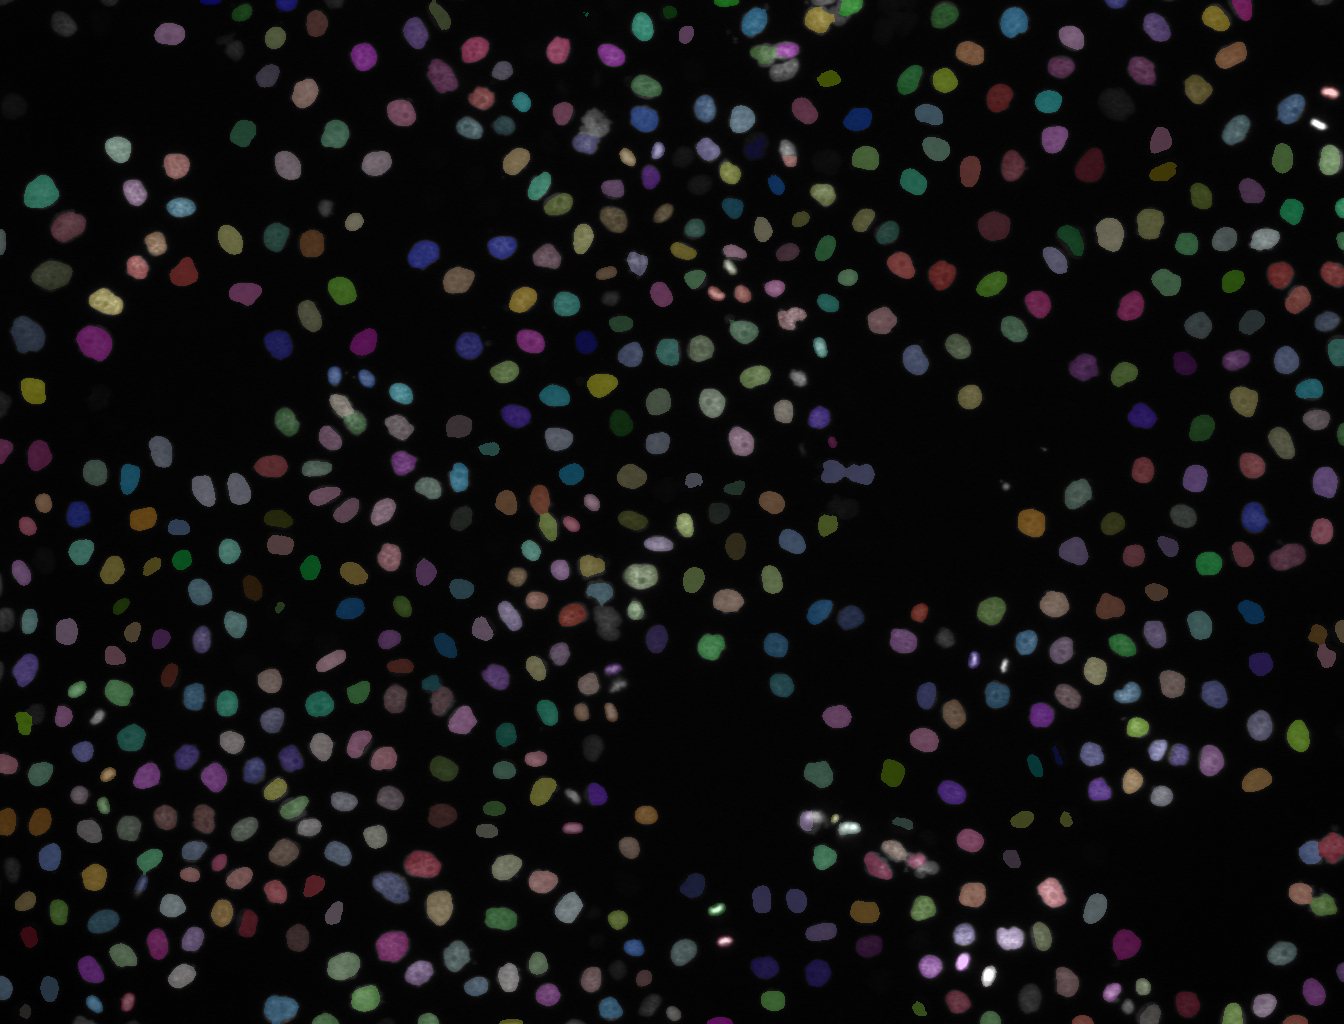
\includegraphics[width=1.0\textwidth]{images/joint/tracking/78_seg_overlay.png}};
            \begin{scope}[x={(image.south east)},y={(image.north west)}]
                \coordinate (c1) at (0.45,0.39);
                \coordinate (c2) at (0.45,0.44);
                \node[thick,draw,ellipse,fill opacity=0,color=red, fit=(c1)
                (c2),scale=0.4,yshift=-1.0mm, opacity=0.7] {};
            \end{scope}
        \end{tikzpicture}
        \caption{$t=78$}
    \end{subfigure}
    \hfill
    \begin{subfigure}[t]{0.3\textwidth}
        \begin{tikzpicture}
            \node[anchor=south west,inner sep=0] (image) at(0,0)
            {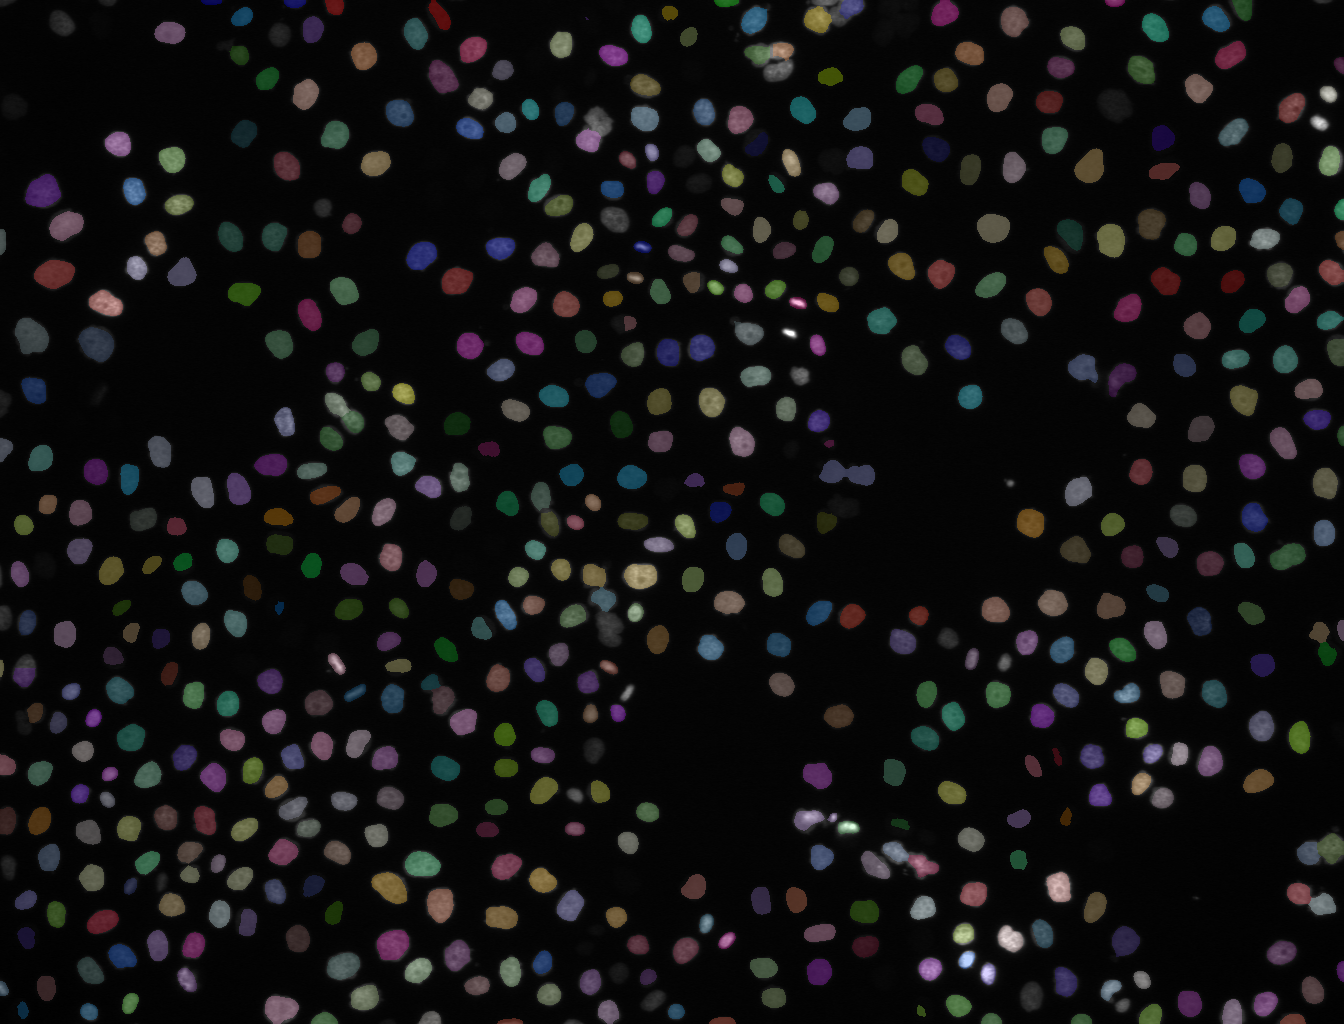
\includegraphics[width=1.0\textwidth]{images/joint/tracking/79_seg_overlay.png}};
            \begin{scope}[x={(image.south east)},y={(image.north west)}]
                \coordinate (c1) at (0.45,0.39);
                \coordinate (c2) at (0.45,0.44);
                \node[thick,draw,ellipse,fill opacity=0,color=red, fit=(c1)
                (c2),scale=0.4,yshift=-1.5mm, opacity=0.7] {};
            \end{scope}
        \end{tikzpicture}
        \caption{$t=79$}
    \end{subfigure}
    \\
    \begin{subfigure}[t]{0.3\textwidth}
        \begin{tikzpicture}
            \node[anchor=south west,inner sep=0] (image) at(0,0)
            {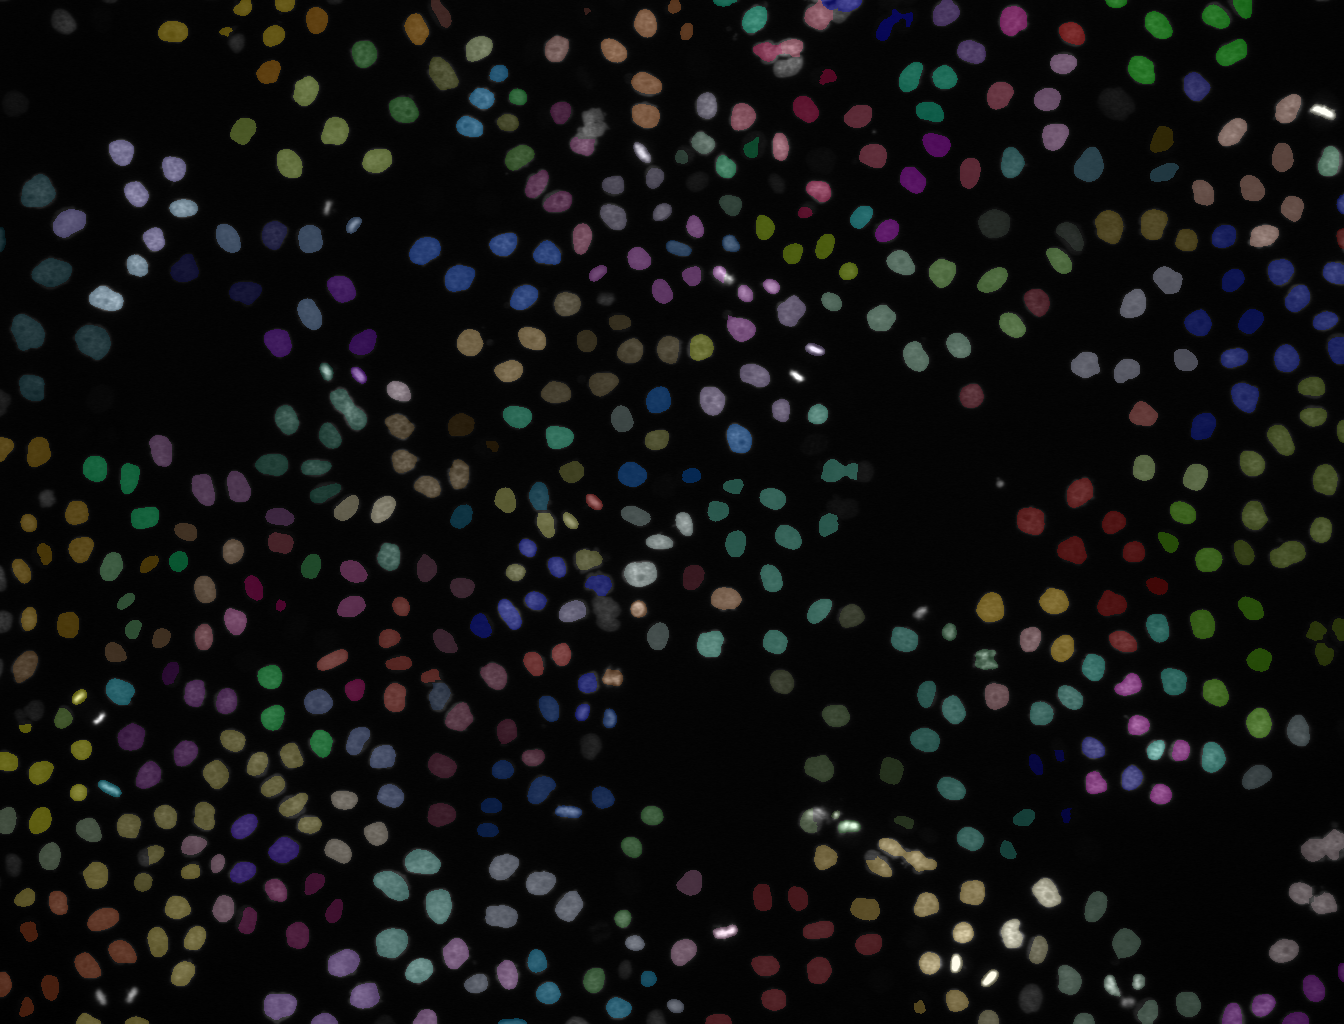
\includegraphics[width=1.0\textwidth]{images/joint/tracking/77_tracking_overlay.png}};
            \begin{scope}[x={(image.south east)},y={(image.north west)}]
                \coordinate (c1) at (0.45,0.39);
                \coordinate (c2) at (0.45,0.44);
                \node[thick,draw,ellipse,fill opacity=0,color=red, fit=(c1)
                (c2),scale=0.4,yshift=-0.5mm, opacity=0.7] {};
            \end{scope}
        \end{tikzpicture}
        \caption{$t=77$}
    \end{subfigure}
    \hfill
    \begin{subfigure}[t]{0.3\textwidth}
        \begin{tikzpicture}
            \node[anchor=south west,inner sep=0] (image) at(0,0)
            {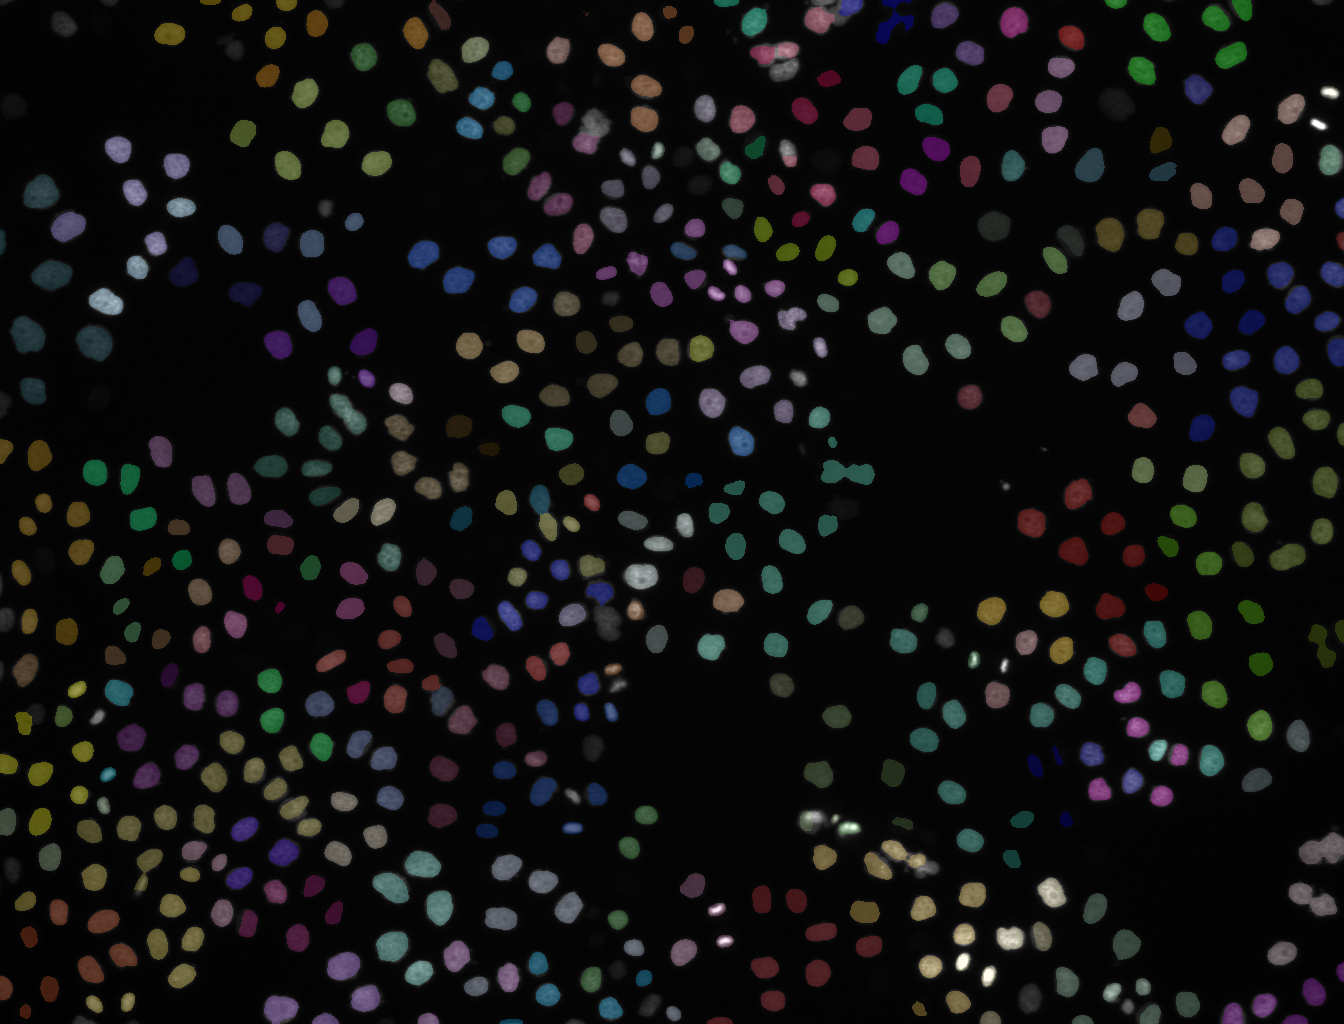
\includegraphics[width=1.0\textwidth]{images/joint/tracking/78_tracking_overlay.png}};
            \begin{scope}[x={(image.south east)},y={(image.north west)}]
                \coordinate (c1) at (0.45,0.39);
                \coordinate (c2) at (0.45,0.44);
                \node[thick,draw,ellipse,fill opacity=0,color=red, fit=(c1)
                (c2),scale=0.4,yshift=-1.0mm, opacity=0.7] {};
            \end{scope}
        \end{tikzpicture}
        \caption{$t=78$}
    \end{subfigure}
    \hfill
    \begin{subfigure}[t]{0.3\textwidth}
        \begin{tikzpicture}
            \node[anchor=south west,inner sep=0] (image) at(0,0)
            {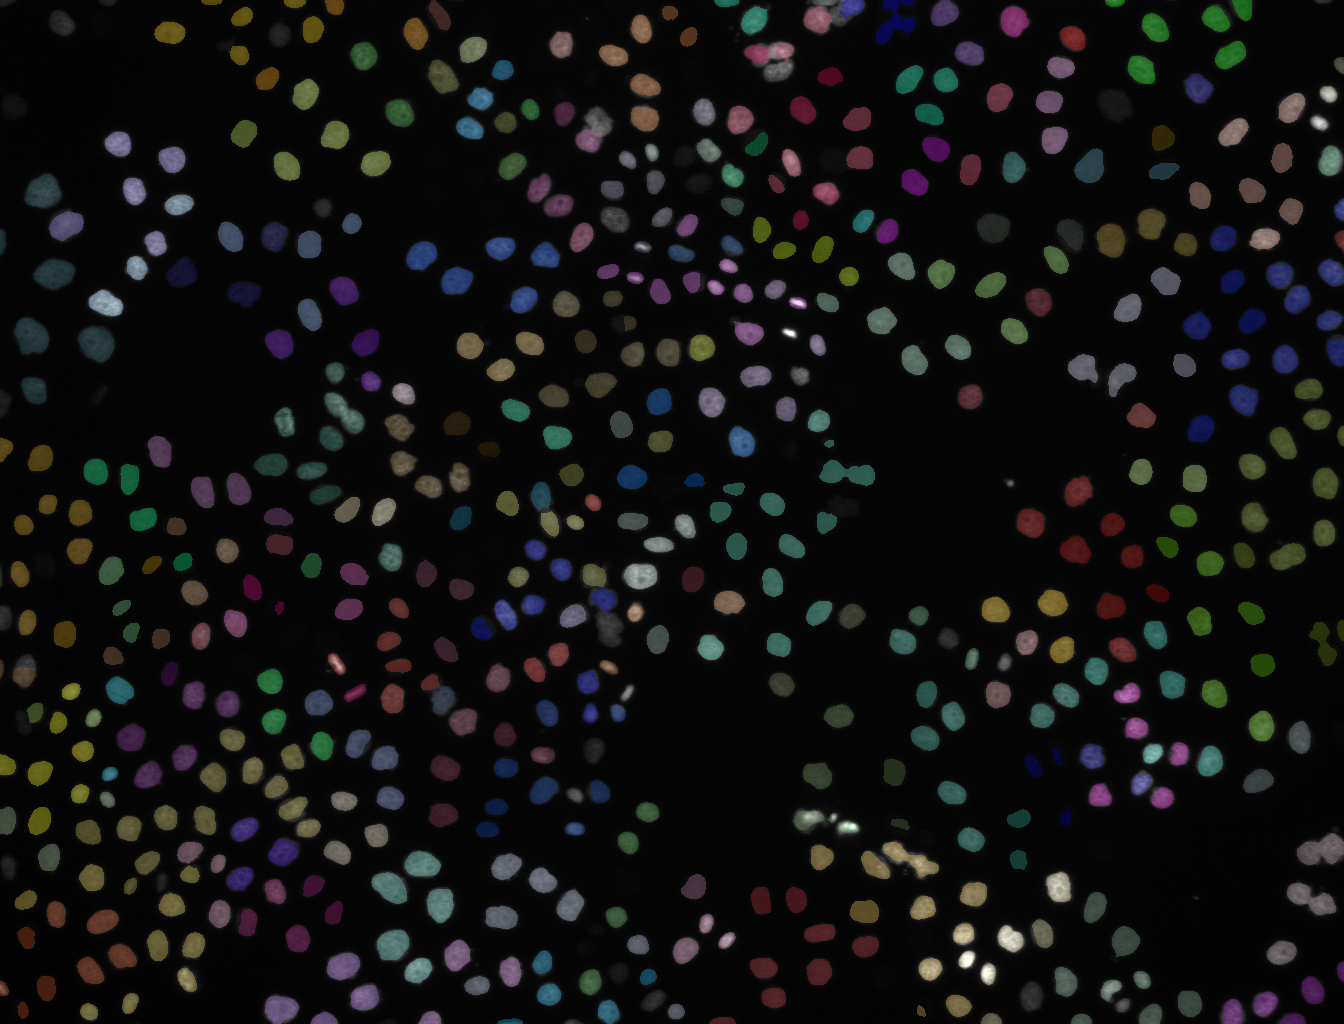
\includegraphics[width=1.0\textwidth]{images/joint/tracking/79_tracking_overlay.png}};
            \begin{scope}[x={(image.south east)},y={(image.north west)}]
                \coordinate (c1) at (0.45,0.39);
                \coordinate (c2) at (0.45,0.44);
                \node[thick,draw,ellipse,fill opacity=0,color=red, fit=(c1)
                (c2),scale=0.4,yshift=-1.5mm, opacity=0.7] {};
            \end{scope}
        \end{tikzpicture}
        \caption{$t=79$}
    \end{subfigure}
    \caption[Joint segmentation and tracking result for three consecutive frames:]{Joint
        segmentation and tracking result for three consecutive frames: $t=77$, $t=78$ and
        $t=79$. The bottom row shows the color coded tracking: In case of a division, the children
        cells take the color of their parent. This leads to ambiguities, when two cells with a
        common ancestor touch at a later stage in the tracking. With the colored tracking alone,
        this case cannot be distinguished from a wrong tracking where the two cells have been
        determined to be one larger cell. Therefore, the top row shows the active regions after
        inference. Here, the two cells in question have different color in case of a correct
        segmentation and tracking, and the same color otherwise. A typical tracking error is marked
        by a red ellipse.}
    \label{fig:joint-tracking-result}
\end{figure}

These illustrative examples have been picked because they demonstrate where joint segmentation and
tracking fails: In case of larger connected components with a higher number of segments, the
tracking tends to disable segments, even if inappropriate.

\newlength\tablemodifiermathheight
\settototalheight\tablemodifiermathheight{\parbox{\linewidth}{$71$}}
\begin{table}
    \centering
    \renewcommand*{\arraystretch}{0.5}
    \begin{tabular}{ccccc}
        $t$ & Raw & Oversegmentation & Connected Component & Tracking \\ \midrule
        $77$ & \raisebox{\tablemodifiermathheight-\height}{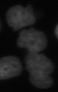
\includegraphics[width=0.15\textwidth]{images/joint/tracking/01/raw_crop.png}}
        & \raisebox{\tablemodifiermathheight-\height}{
\includegraphics[width=0.15\textwidth]{images/joint/tracking/01/layer_00_crop.png}}
        & \raisebox{\tablemodifiermathheight-\height}{
\includegraphics[width=0.15\textwidth]{images/joint/tracking/01/layer_04_all_crop.png}}
        &
        \raisebox{\tablemodifiermathheight-\height}{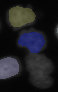
\includegraphics[width=0.15\textwidth]{images/joint/tracking/01/77_tracking_overlay_crop.png}}
        \\ &&&& \\
        $78$ & \raisebox{\tablemodifiermathheight-\height}{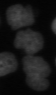
\includegraphics[width=0.15\textwidth]{images/joint/tracking/02/raw_crop.png}}
        & \raisebox{\tablemodifiermathheight-\height}{
\includegraphics[width=0.15\textwidth]{images/joint/tracking/02/layer_00_crop.png}}
        & \raisebox{\tablemodifiermathheight-\height}{
\includegraphics[width=0.15\textwidth]{images/joint/tracking/02/layer_04_all_crop.png}}
        &
        \raisebox{\tablemodifiermathheight-\height}{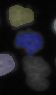
\includegraphics[width=0.15\textwidth]{images/joint/tracking/02/78_tracking_overlay_crop.png}}
        \\ &&&& \\
        $79$ & \raisebox{\tablemodifiermathheight-\height}{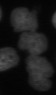
\includegraphics[width=0.15\textwidth]{images/joint/tracking/03/raw_crop.png}}
        & \raisebox{\tablemodifiermathheight-\height}{
\includegraphics[width=0.15\textwidth]{images/joint/tracking/03/layer_00_crop.png}}
        & \raisebox{\tablemodifiermathheight-\height}{
\includegraphics[width=0.15\textwidth]{images/joint/tracking/03/layer_04_all_crop.png}}
        &
        \raisebox{\tablemodifiermathheight-\height}{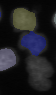
\includegraphics[width=0.15\textwidth]{images/joint/tracking/03/79_tracking_overlay_crop.png}}
        \\ &&&& \\
        \bottomrule 
    \end{tabular}
    \renewcommand*{\arraystretch}{1.0}
    \caption[A single connected component with falsely deactivated regions]{A single connected component with falsely deactivated regions (no intermediate regions
        were merged from the segments). The same cluster of cells is shown over three time steps with the according segmentation showing that an
        activation of more regions would have been reasonable. However, the factor graph decided to
        turn off some of the cell-like regions. In an optimal tracking, the lower part of the merged
        object in the middle would be active.}
    \label{tab:joint-tracking-result}
\end{table}

% In addition and due to the lack of a gold standard, the tracking result has been evaluated by manual
% inspection. A random selection of events both in ground truth and tracking result form the basis for
% comparison. The results are summarized in \cref{tab:joint-result-numbers}.
The ground truth used for evaluation of the conservation tracking method in
\cref{sec:gmm-experiments} is based on the segmentation that was used for tracking and thus cannot
be used as a gold standard in the joint tracking and segmentation.  Therefore,
\cref{tab:joint-result-numbers} shows the results of a manual evaluation of a selection of cells
compared to raw data by visual inspection. For that purpose, $317$ moves have been randomly selected
from each of raw data and tracking result. For the divisions, a random subset of $100$ and $87$
events has been picked from tracking result and raw data, respectively. Randomness is injected by
random sampling from the events on the tracking result side, and by choosing the event that is
closest to a randomly sampled tuple of time step and coordinates in case of raw data events.

In a strict measure for move events, moves are considered false moves if they connect regions that
either exceed one and a half times of, or fall below half the size of the corresponding cell in raw
data. On the contrary, in a relaxed measure, these moves fall in the true positive category, \cf the
rows starting with \emph{Moves} in \cref{tab:joint-result-numbers}. Similarly, divisions are off by
one or two time steps compared to raw data in many cases. Therefore, an additional, more tolerant
measure for divisions is applied, which considers a division true positive, if the
corresponding raw data division occurs within a range of two time steps, \cf the rows starting with
\emph{Divisions} in \cref{tab:joint-result-numbers}. Note that, in contrast to mitosis detection and
without exception, a division is only true positive, if all three involved cells, \ie parent and
child cells, are detected correctly.



The results in \cref{tab:joint-result-numbers} confirm that the overall tracking result looks
promising. The lower recall for moves in comparison to precision indicates that the tracking falsely
deactivates too many regions. Furthermore, the discrepancy between strict and tolerant division
measures implies that a better division classifier could improve tracking results. Still, even with
the more tolerant measures, there is room for improvement, as the aforementioned problem of falsely
deactivated regions persists. In the following, we identify the reasons for these shortcomings and
justify future work and enhancement of the model.

\begin{table}
    \centering
    \begin{tabular}{l|ccc}
        \toprule
        & Precision & Recall & $\fmeasure$ \\ \hline
        Moves - size filter\tablefootnote{A move is only true positive if both involved regions are larger
            than half the size and smaller than 1.5 times the size of the the cell in raw data.} & 0.970 & 0.901 & 0.934 \\
        Moves - no size filter\tablefootnote{The size filter for regions that are involved in moves
            is not applied.} & 0.979 & 0.921 & 0.949 \\
        Divisions - strict\tablefootnote{If a division occurs at a time shifted by one or two compared to
            raw data, it is considered a wrong event.} & 0.654 & 0.654 & 0.654 \\
        Divisions - tolerant\tablefootnote{Divisions have a time step tolerance of $2$.} & 0.890 & 0.825
        & 0.856 \\
        \bottomrule
    \end{tabular}
    \caption[Joint segmentation and tracking results]{Joint segmentation and tracking results for
        data set C (\cref{subsec:gmm-data}) based
        on evaluation by visual inspection. Precision, recall and $\fmeasure$
        (\cref{subsec:gmm-measures}) are used for evaluation of the data. We present both strict and more
        tolerant evaluation schemes for moves and divisions.}
    \label{tab:joint-result-numbers}
\end{table}



\subsection{Continuation of the Work on the Model}
\label{subsec:joint-continuation}
As demonstrated in the previous sections, joint segmentation and tracking suffers from tracking
errors in the presence of connected components with many segments. More specifically, regions
corresponding to actual cells are deactivated in the tracking. However, the active regions in the
final result still constitute a meaningful tracking with the limitation that divisions appear one or
two time steps too early in many cases. Thus, the task for ongoing work on the model is to modify
the method in a way that pushes the result towards activating these falsely deactivated regions.

Due to the complexity of the method, locating the weak spots is essential. To begin with, the
initial oversegmentation seems reasonable. As demonstrated in
\cref{fig:joint-experiment-overseg-a,fig:joint-experiment-overseg-b}, the initial segments
either oversegment or exactly fit single cells in most cases. Furthermore,
\cref{tab:joint-region-merging-examples} shows that the region merging works well by producing a
richer set of cell-like regions. A more sophisticated merging algorithm would not fundamentally
change the tracking result. However, learned edge weights based on the output of the region
classifier~(\cref{sec:joint-classifier-Region}) could easily be implemented into the workflow
and would give a more reasonable basis for the classifier decision.

On the other hand, the factor graph wrongly decided to turn off regions and, in many cases,
inferred divisions one time step too early. Thus the error occurs in the creation of the
hypotheses or during inference and these steps need to be revised with the following approaches
promising positive results:

To begin with, the pruning of potential assignments (\cref{subsec:joint-hypotheses-graph}) may be too
restrictive and discard assignment hypotheses, which would have turned out to be true. Take two
connected components $c^t$ and $c^{t+1}$ at times $t$ and $t+1$, respectively, each consisting
of two segments. If the displacement of the connected components is large enough, both conflict
sets in $c^t$ might have the same conflict set in $c^{t+1}$ for their nearest neighbor. In that
case, inference would tend to falsely disable regions without incoming assignment hypotheses,
even if it contradicts the actual events in raw data. A solution to this problem could be a less
restrictive pruning algorithm. This could be achieved by finding more than one nearest neighbors
for each conflict set. However, with a nearest neighbor search only in forward direction in
time, the potential loss of regions persists. Therefore, a single nearest neighbor should be
searched both forward and backward in time. In this, all regions have incoming assignment
hypotheses, unless the encompassing connected component does not have any incoming arcs in the
hypotheses graph.

Moreover, the division classifiers tend to predict divisions one time step too early. The obvious
answer to this issue is a retraining of the division classifiers. For a definite evaluation of the
classifiers, their output needs to be visualized. Due to the prediction for all possible divisions
of a cell, this turns out unmanageable. A reasonable approximation is the probability of the most
likely division. In the corresponding visualization, cells take values according to the maximum
division probability. With an appropriate color map, \eg gray scale or jet\footnote{Low and high
    values are represented by blue and red color, respectively,
    \\\cf\url{http://wiki.scipy.org/Cookbook/Matplotlib/Show_colormaps}.}, the classifier prediction
can be efficiently compared to the tracking result and the source of the early divisions can be
located at either of the division classifier or the graphical model.

Finally, bugs in the code cannot be excluded as a source for problems. Thus a revision of the code
is necessary. In order to analyze the behavior of the model and the effects of potential solutions
to the existing problems, and to fix potential bugs, a small subset of representative cells should
be cropped from raw data. The sample should be sufficiently small to allow for a manual reproduction
of the factor graph and inference. Furthermore, these examples with the desired results should serve
as unit tests in addition to existing ones.

A more radical approach would be a complete revision of the graphical model in conjunction with a
disposal of the region merging. Then, based on the initial oversegmentation, the graphical model
would decide, which segments should be merged into larger regions. This, however, would require
multi-state random variables and higher order factors that manage the grouping of segments into
larger regions and enforce additional consistency constraints, \eg regions must be connected. In
addition to this explosion of the model, the labeling would be ambiguous: Labeling one region $1$
and another region $2$ is equivalent to setting the labels the other way round. Therefore, although
this approach is really interesting in theory, in practice it would not be tractable. An even more
extreme effort would be a complete omission of the initial segmentation and building the factor
graph on the pixel level. However, it is obvious that this problem is not tractable by any means due
to its huge size.

In summary, we proposed a method that jointly optimizes segmentation and tracking as an approach to
handle undersegmentation in cell tracking, and thereby goes beyond existing tracking-by-assignment
methods~(\cref{fig:joint-pipeline}). First, a set of possibly competing segmentation hypotheses is
generated~(\cref{sec:joint-oversegmentation}). Then, the factor graph chooses those segmentations
that constitute the most meaningful tracking result~(\cref{sec:joint-graphical-model}). To this end,
discriminative classifiers for count, regions, divisions and moves~(\cref{sec:joint-classifiers})
implement local evidence in the factors. Finally, experiments in \cref{sec:joint-experiments} show
promising results that suggest a continuation of the work on the model in order to solve the
existing issues~(\cref{subsec:joint-continuation}).

%%% Local Variables: 
%%% mode: latex
%%% TeX-master: "../../../main"
%%% End: 
